\chapter{流量检测系统的设计与实现}
\section{引言}
本章结合前四章的分析和结论,将基于特征关系图的RNN模型应用到实际流量环境中,验证其真实有效性。因此本文针对清华大学校园网的流量环境,设计了一个流量异常检测系统。该系统应该满足以下几点要求:
\begin{enumerate}
  \item 实时性。如果一个系统检测延迟很高,那么即使其准确率同样很高,这个检测结果也将毫无意义。因为异常检测的目的是在攻击的早期阶段就将其发现,并且作出应对。
  \item 高效性。校园网用户规模大,流量峰值高,该系统需要能够高效处理海量的流量数据。
  \item 鲁棒性。该系统应该保证能够在复杂的网络环境面前依然有较好的检测效果,例如发生突出事件或者新的异常类型时依然能够有一定的检测效果。
  \item 可扩展性。该系统的各个模块之间的耦合度应尽可能低,一方面便于调试,另一方面可以便捷的验证其他算法模型。
\end{enumerate}

本文的流量异常检测系统按照上述需求设计如图\ref{fig:arch}所示,可以分为三个模块:输入模块,模型模块,输出模块。其中输入模块将流量数据和SOC标签数据整合成特征数据;模型模块分为离线训练和在线检测两部分,离线训练部分定期产出更新好参数的模型,在线检测部分会接受当前的特征数据进行判别;最后输出模块将判别结果根据历史信息进行异常等级划分,给运维人员下一步提供参考。
% TODO: 图中加入关系矩阵
\begin{figure}
    \centering
    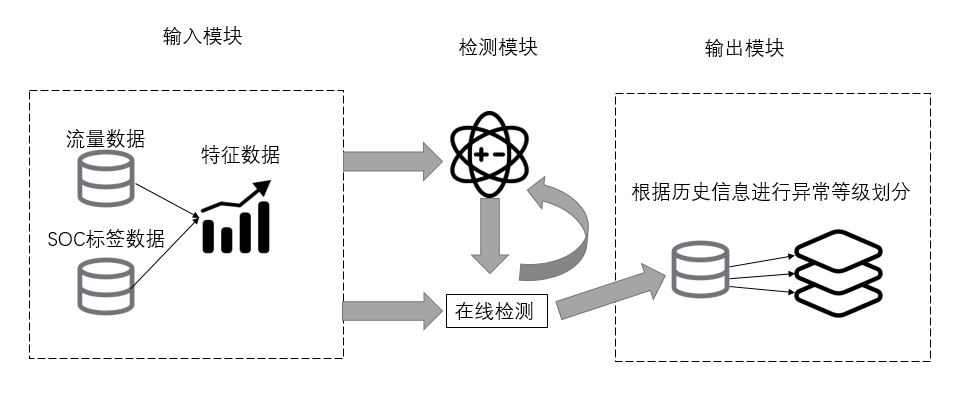
\includegraphics[scale=0.55]{系统架构图.png}
    \caption{系统架构图}
    \label{fig:arch}
  \end{figure}


\section{spark 平台介绍}
Apache Spark是由UC Berkeley AMP Lab开源的用于大规模数据处理的统一分析引擎\cite{spark},现如今已经成为Apache软件基金会的最为出名的开源项目之一。Spark原理与Hadoop类似,都是基于MapReduce进行分布式计算,但是功能更加丰富,且支持SQL查询、流式处理、图计算等功能。

Spark具有以下几个特点:

\begin{itemize}
  \item 速度快。这是因为Spark基于内存计算,而Hadoop MapReduce必须进行读取和写入磁盘,IO操作比内存操作更加耗时。图\ref{fig:Logistic regression in Hadoop and Spark}是Spark官网给出的一项逻辑回归任务在Hadoop和Spark两个系统的运行时长对比。
   \begin{figure}
    \centering
    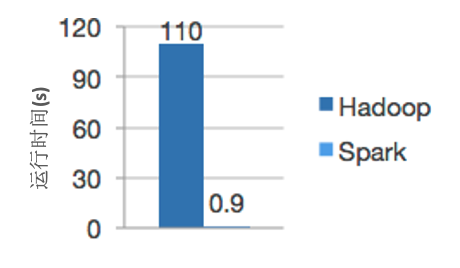
\includegraphics[width=0.3\linewidth]{logistic-regression.png}
    \caption{Logistic regression in Hadoop and Spark}
    \label{fig:Logistic regression in Hadoop and Spark}
  \end{figure}
  \item 易用性。Spark提供了80余种高级API,可以轻松编写高度并行的应用程序。Spark支持Java, Scala, Python, R, and SQL等多种编程语言。
  \item 兼容性。Spark支持多种数据源作为输入,例如本地文件系统、HDFS、HBase等,并且Spark支持多种运行模式,能够做到类似java的“一次编写,多处运行”。
\end{itemize}



如图\ref{fig:Spark组件}所示,Spark项目包含多个独立组件。其最核心的模块为深蓝色的Spark Core,其定义了核心API,如“弹性分布式数据集”,该模块也负责调度、监控计算集群中的计算任务,具有内存管理,故障恢复,与管理系统、存储系统交互等功能。为了满足分布式计算系统的可扩展性,Spark支持在各种集群管理器之上运行,例如图中灰色的模块Hadoop YARN,Apache Mesos以及浅蓝色的Spark系统中包含的“独立调度程序”(Standalone Scheduler)。在Spark Core之上,具有浅蓝色的四个组件:Spark SQL(处理结构化数据),Spark Streaming(实时处理海量数据),MLlib(运行机器学习模型),GraphX(提供图计算)。本文中的系统主要使用Spark Streaming组件。



\begin{figure}
  \centering
  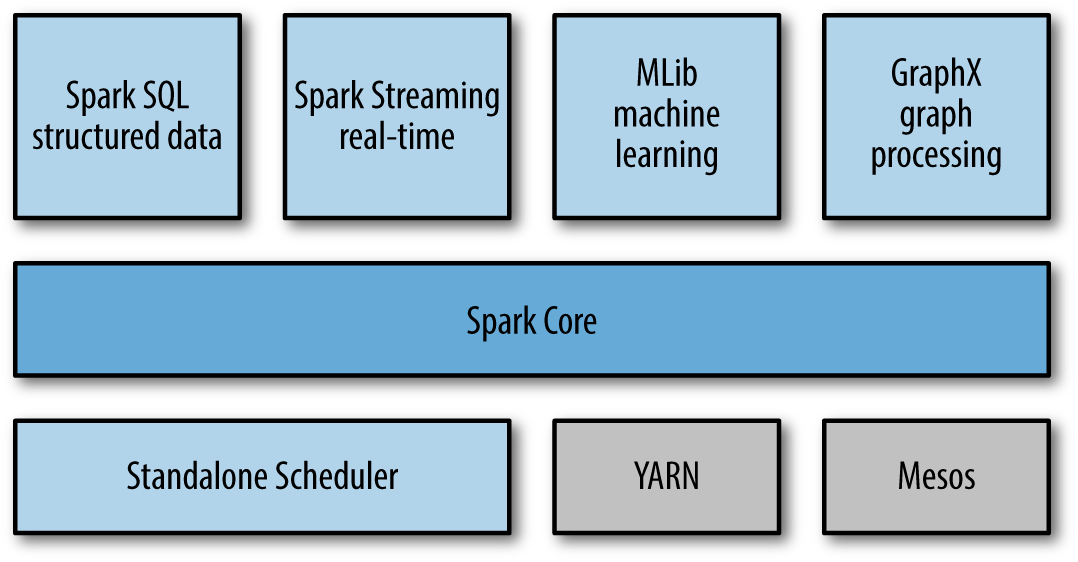
\includegraphics[width=0.6\linewidth]{spark-stack.png}
  \caption{Spark组件}
  \label{fig:Spark组件}
\end{figure}

图\ref{fig:spark工作原理}是
\begin{figure}
  \centering
  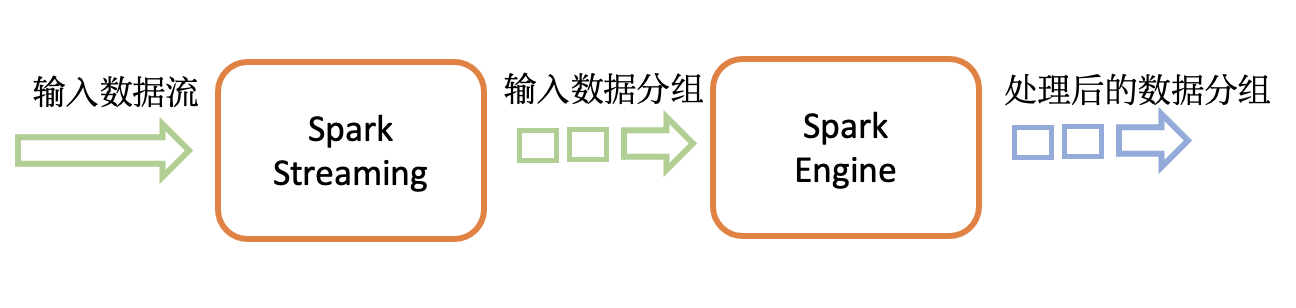
\includegraphics[scale=0.6]{spark工作原理.png}
  % 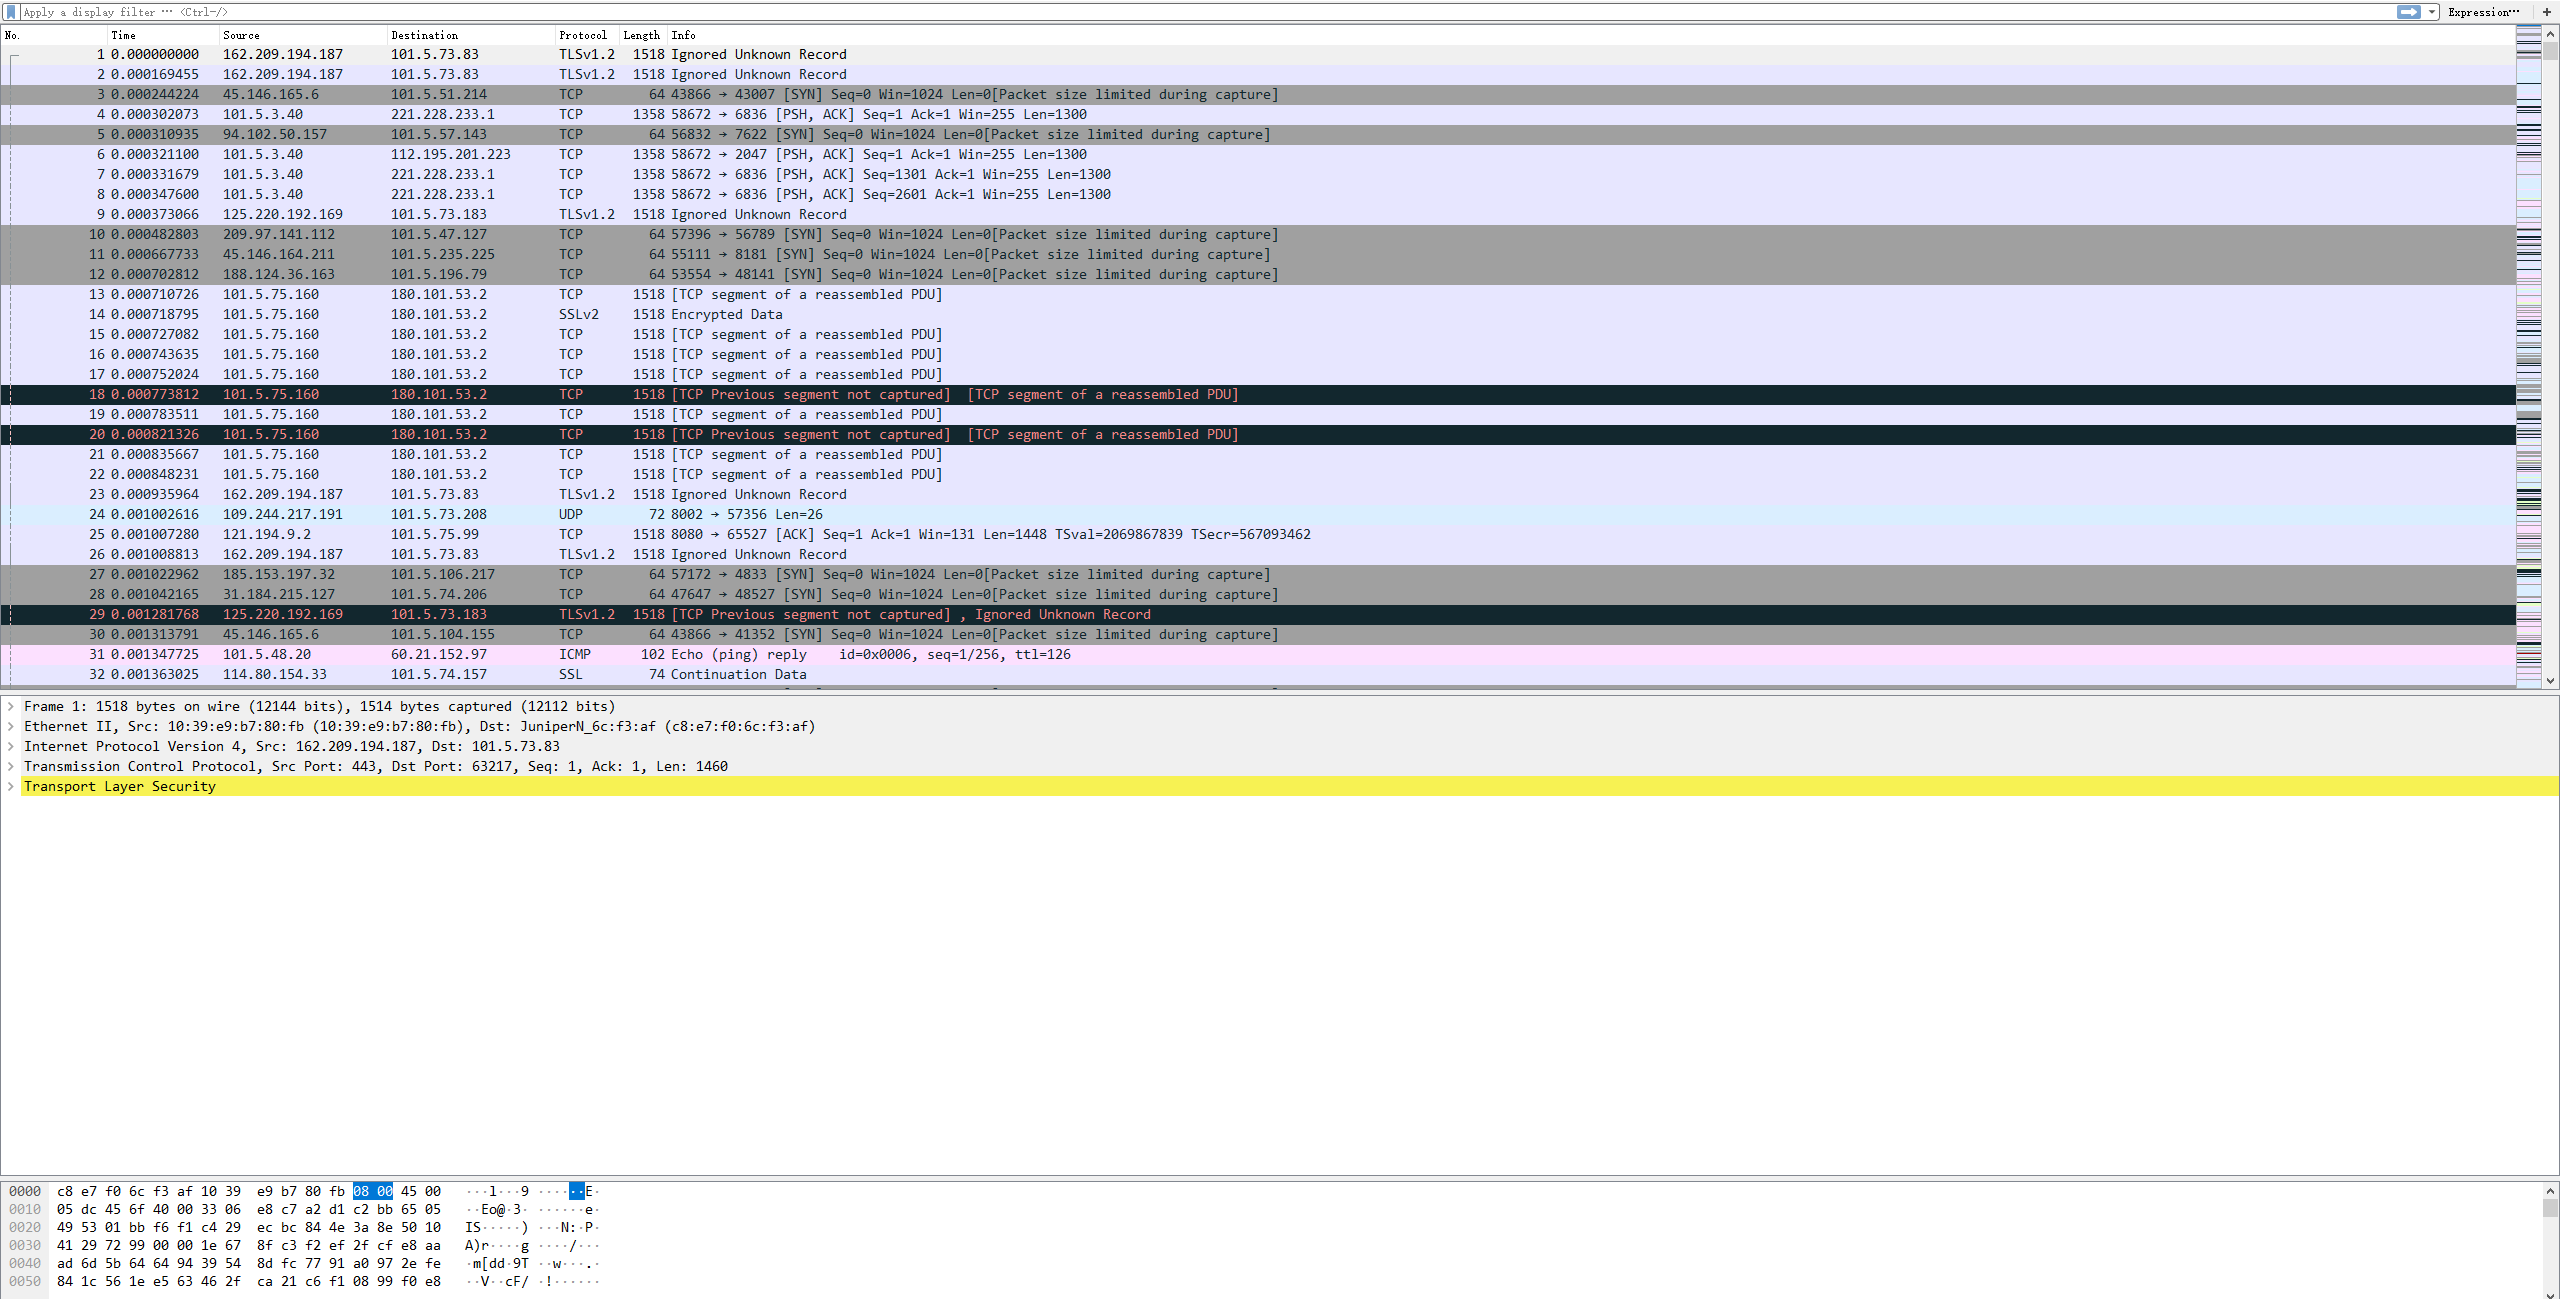
\includegraphics[width=0.6\linewidth]{wireshark流量图.png}
  \caption{spark streaming工作原理}
  \label{fig:spark工作原理}
\end{figure}

\section{系统架构与实现}
本文实现流量异常检测系统的架构如图\ref{fig:arch}所示,整个架构是基于Spark Streaming实现。本节将分模块具体介绍。
\subsection{输入模块}
输入模块的主要功能是对流式数据进行特征抽取,与第三章中的特征提取单一文件不同的是,本模块处理的数据是“无界”的。我们需要将无界数据进行切片,每次处理一个片段内的数据。这些片段又被称为“window”,window是流式计算领域的核心概念。

本模块的输入为由kafka传入的流量数据,然后将流量报文划分到一个个滑动窗口(sliding window)中,每次处理一个窗口内的全部报文。流量特征提取的整体流程图\ref{fig:特征提取}所示。读取到packet后,首先为每条报文建立一个由五元组信息组成的标志,然后根据图中的规则依次判断该报文是否是一条新的流的起始报文、是否是当前流的结束报文、是否需要调用updateflow更新各项统计信息。

\begin{figure}
  \centering
  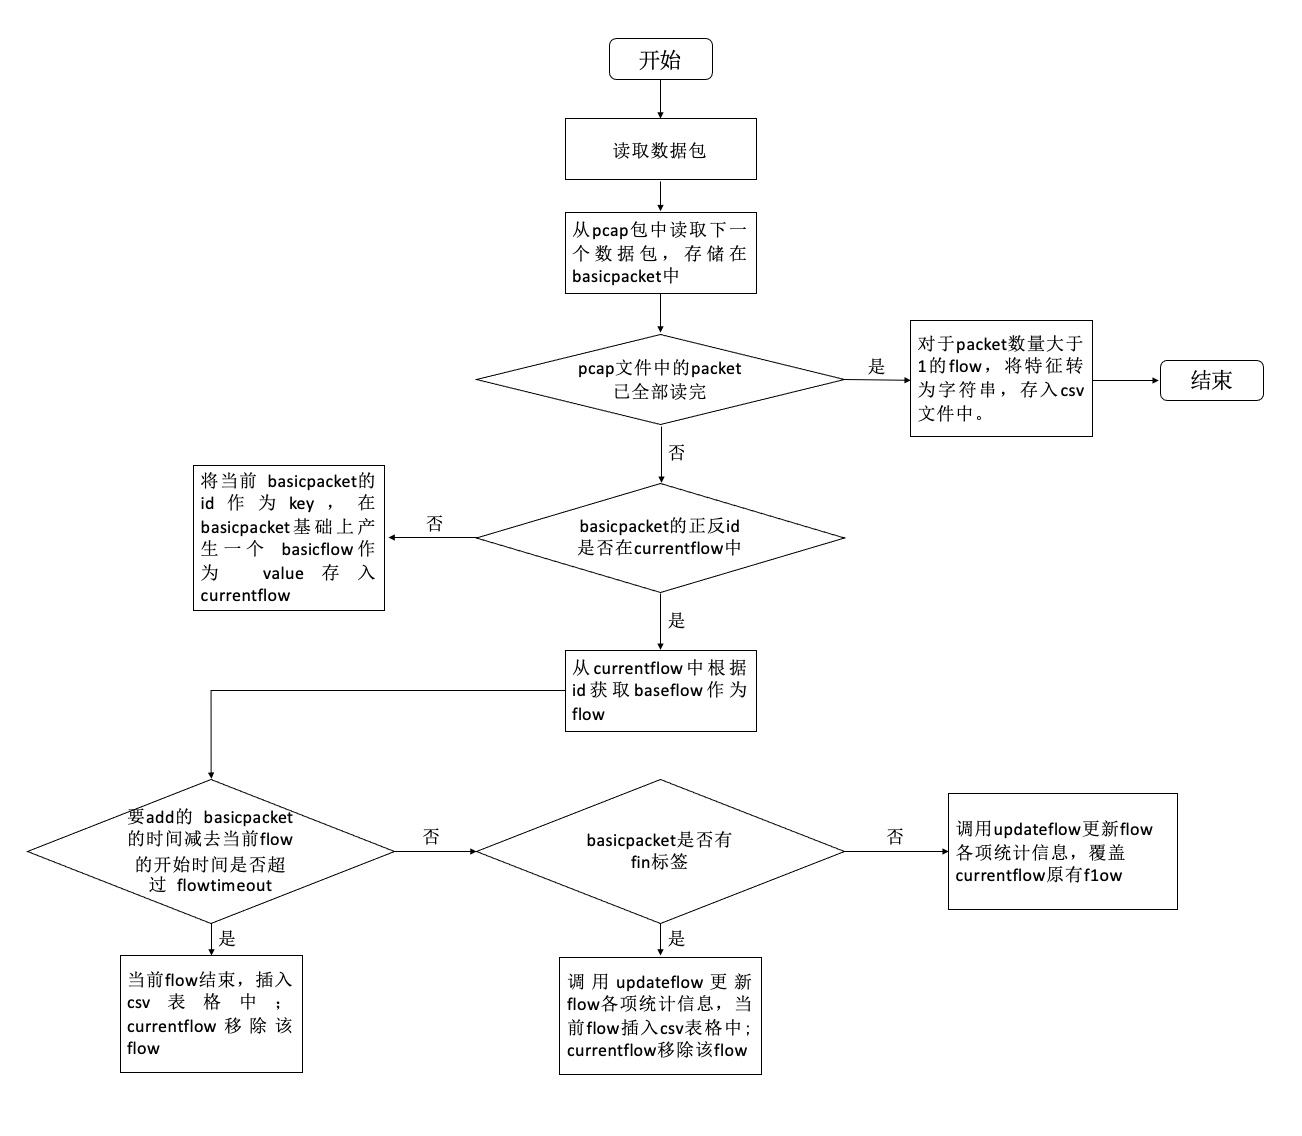
\includegraphics[scale=0.3]{特征提取.jpg}
  \caption{特征提取}
  \label{fig:特征提取}
\end{figure}

本模块提取的结果是以一条TCP流或者UDP流为单位,该条流中全部报文的统计信息。在一条流中有很多个数据包,TCP流以三次握手为开始,以FIN标志为结束;UDP流以首次出现为开始,以超出超时时间为结束。并且每条流都是双向数据流,由源ip地址到目的ip地址为正向,目的ip地址到源ip地址为反向。

使用该方法得到的csv文件如图\ref{fig:特征文件}所示:
\begin{figure}
    \centering
    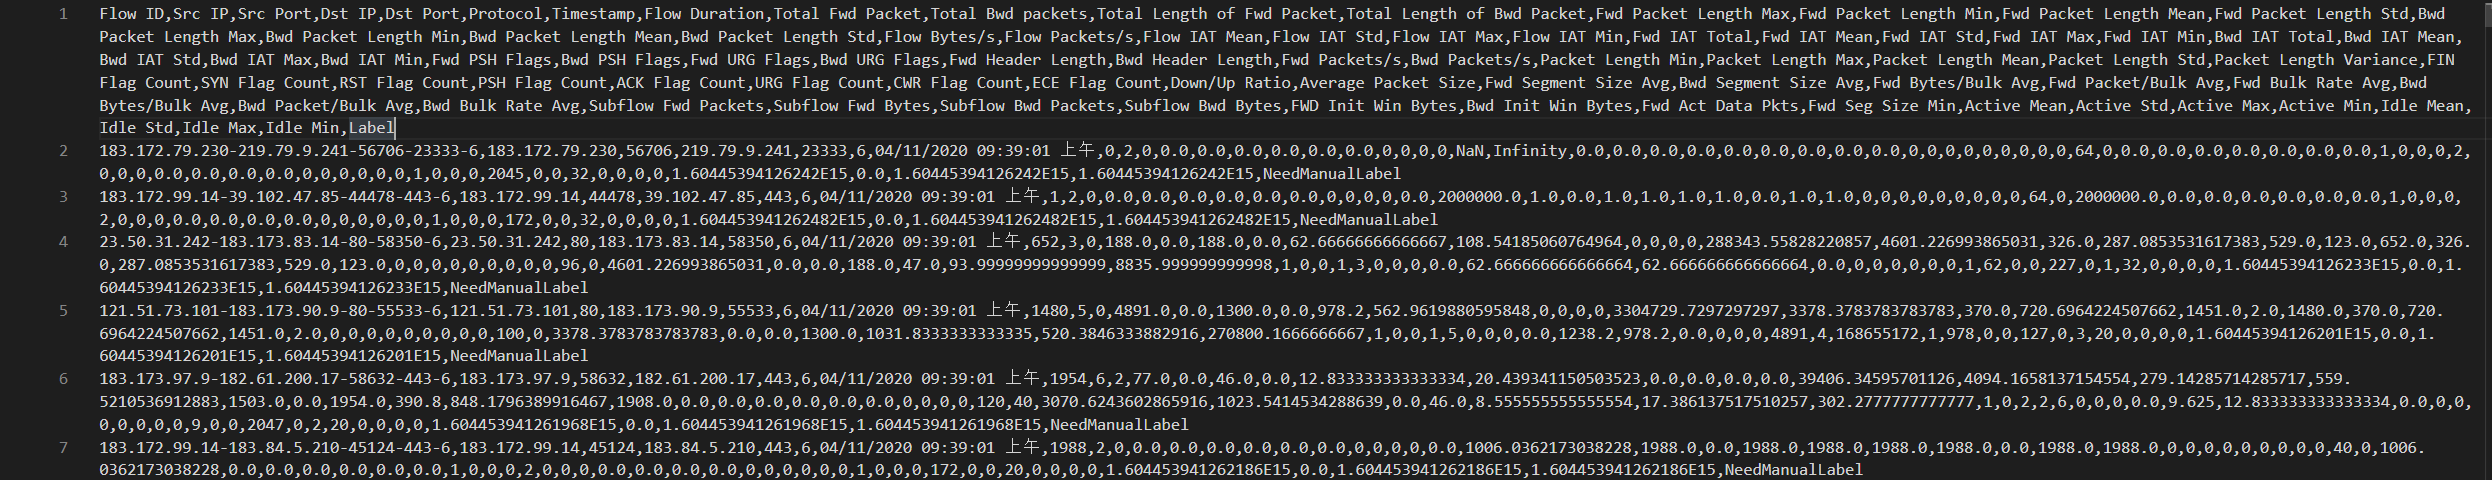
\includegraphics[scale=0.2]{特征文件.png}
    \caption{特征文件}
    \label{fig:特征文件}
  \end{figure}


\subsection{检测模块}
检测模块分为离线和在线两部分,并且由于第四章中FG-RNN算法的特点,特征关系图(Feature Graph)的更新频率与循环神经网络(RNN)不同,并且这两者在实现中已经解耦,因此RNN的参数更新仅需在离线部分完成,在线部分可以兼顾实时流量的检测和特征关系图参数的更新。

\subsection{输出模块}
在得到实时检测模块给出的异常流信息以及类型后,我们可以基于此做出进一步的处理。由于校园网流量“异常是常态,甚至半数流量是异常”的特点,若将全部异常信息都汇报给运维人员,大量危害程度低的异常告警势必会掩盖真正值得关注的异常,例如时刻都在发生的网络扫描,由于其重要性低微我们可以将其忽略。

因此,我们需要对异常的重要等级进行评分,具体地评分规则如下:首先初始化每种异常类型的基础分数,将异常分为低危、中危、高危三类,然后每次运维人员处理一条异常流后,将发现该流异常到处理异常的时间差作为权重,重新计算该异常的评分。



% \begin{figure}
%     \centering
%     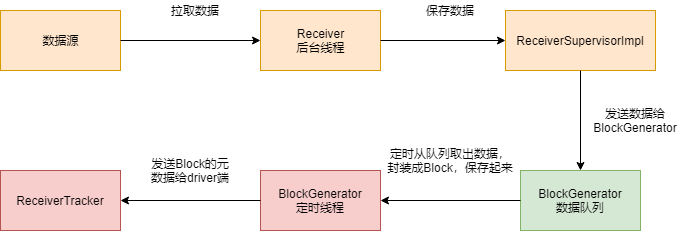
\includegraphics[scale=0.6]{spark数据源.png}
%     \caption{Spark数据源}
%     \label{fig:spark}
%   \end{figure}

% \section{流式数据特征抽取}
% Spark Streaming 支持 Scala、Java 和 Python,本文中使用Python提交任务。使用第三章中的特征提取方法,
% 输入为由kafka传入的流量数据,提取的结果都是传输层的一些统计信息,以一个TCP流或一个UDP流为一个单位。TCP流以FIN标志为结束,UDP以设置的flowtimeout时间为限制,超过时间就判为结束。在一个TCP流中有很多个数据包,先三次握手而后传输信息再四次挥手。统计一个流中的统计信息作为提取的特征。且统计的特征都分前后向,规定由源地址到目的地址为正向,目的地址到源地址为反向,例如某条TCP流的源ip地址为192.168.31.100,源端口号为174,目的ip地址为183.232.231.174,目的端口号为443,则为该流构建一个标志叫Flow ID:192.168.31.100-183.232.231.174-46927-443-6,由源地址、目的地址、源端口、目的端口、协议号组成。
% 流量特征提取的整体流程图如下:

% \begin{figure}
%     \centering
%     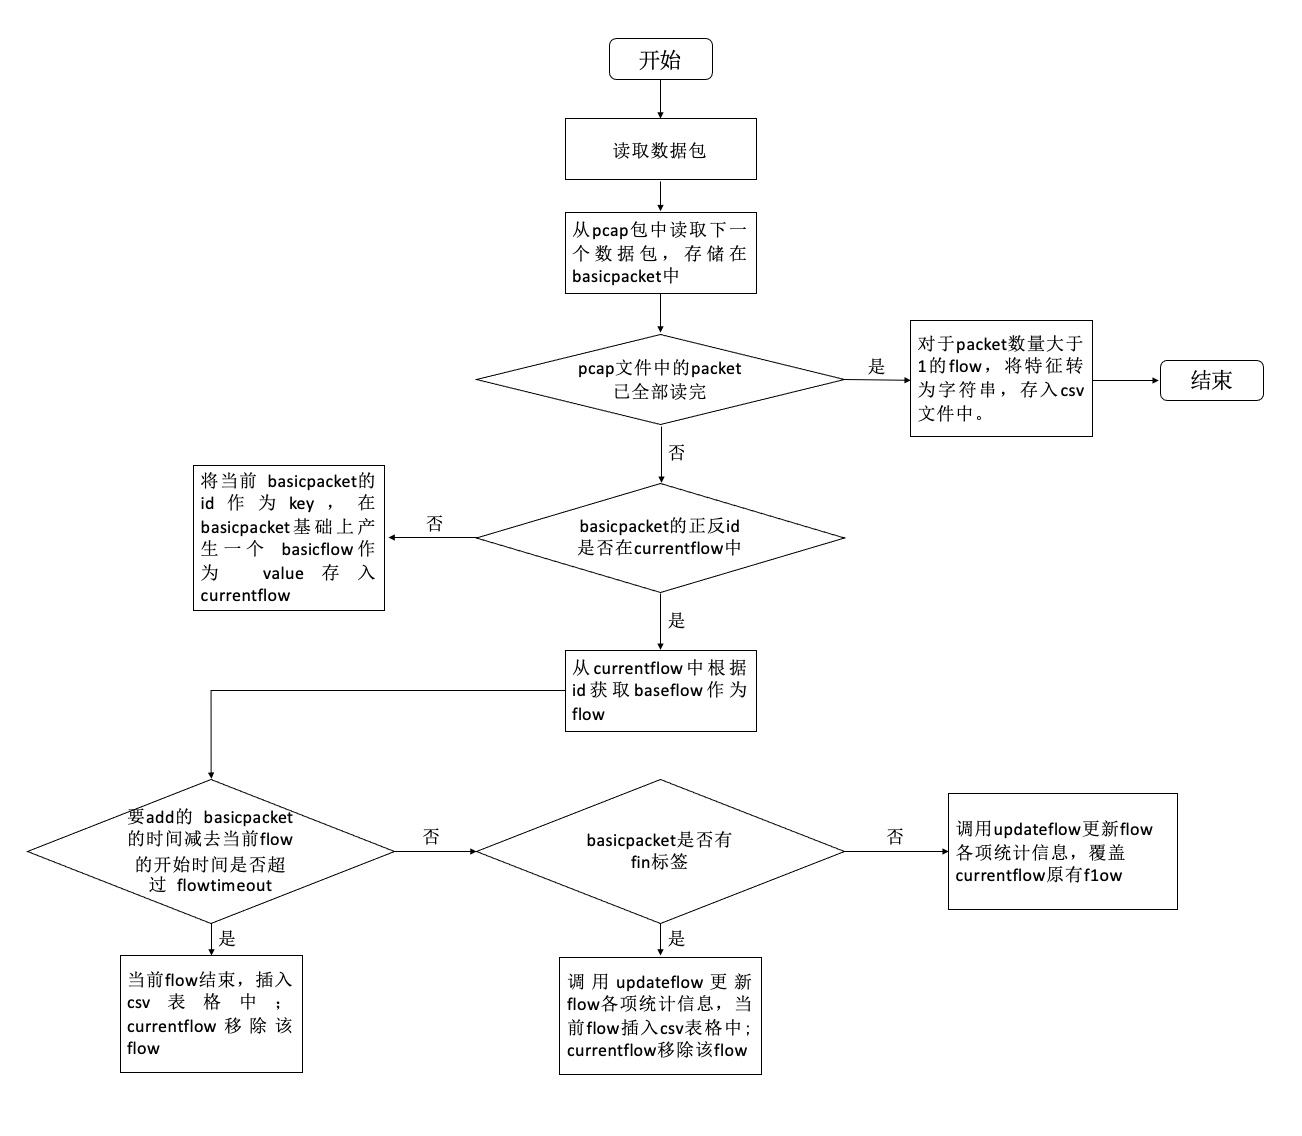
\includegraphics[scale=0.3]{特征提取.jpg}
%     \caption{特征提取}
%     \label{fig:特征提取}
%   \end{figure}


% 在currentFlows存储当前还未结束的所有TCP、UDP流。在添加的过程中不断地更新每个流的统计特征,最终将统计特征写入csv文件。判断新加入的数据包是否属于当前所有未结束的流,如果属于当前流则判断正向还是反向,之后判断时间是否超时、不超时则判断是否含有FIN标志,如果两者都不满足,则声明一个BasicFlow对象,根据id从currentFlows中拿到与当前数据包对应的流,调用addPacket将该数据包加入到对应流中。如果前面判断不在当前所有未结束的流中,则直接创建一个新的流,里面只含当前数据包,存入到currentFlows中。如果属于当前某个未结束的流,且超时或存在FIN标志,则说明当前flow结束,超时则从currentFlows中移除对应流,新建flow存入currentFlows中,含FIN标志则直接从currentFlows中移除对应流。结束的flow直接调用onFlowGenerated函数将流打印存储起来。




% \section{模型训练模块的设计与实现}
% 补充一些图
% \begin{figure}
%   \centering
%   
\includegraphics[width=0.6\linewidth]{example-image-a.pdf}
%   \caption{Example figure in appendix}
%   % \label{fig:appendix-survey-figure}
% \end{figure}
% \section{预测输出模块}
\section{系统结果展示与分析}
本节的目标是建立一个实时、高效、鲁棒、可扩展的流量异常检测系统,因此实验评估需要针对大规模流量场景,尽可能达到压力测试的效果。
本节使用了第3章中CAMPUS数据集的第二段持续时长为18小时的数据作为系统的输入,经过测试,我们发现平均延迟3分钟即可将每个数据包的特征提取到相应的TCP/UDP流中,得到流的特征信息后,实时检测模块可以在1秒内输出异常类型。这得益于离线模型的定期更新。此外,我们还分析了该模型的失效时间,每次更新完一次模型的参数,可以看到随着时间的增长,模型效果越来越差,在5小时后准确率会低于78\%。